\documentclass{article} 
\usepackage{amsmath}
\usepackage{fancyhdr}
\usepackage{geometry}
\usepackage{setspace}
\usepackage{graphicx}
\usepackage[acronym,nonumberlist]{glossaries}
\usepackage[export]{adjustbox}
\usepackage{helvet}
\renewcommand{\familydefault}{\sfdefault}
\graphicspath{ {./figures/} }

\geometry{a4paper, margin=1in}
\onehalfspacing
\thispagestyle{fancy}
\title{Transcriptomic investigation of sleep deprivation in the hippocampus of the mouse}
\author{Zeru Peterson}

% the nonumberlist in the \usepackage and printglossary calls prevents printing page number of usage
\newacronym{ca1}{CA1}{Cornu ammonis subfield 1}
\newacronym{ca2}{CA2}{Cornu ammonis subfield 2}
\newacronym{ca3}{CA3}{Cornu ammonis subfield 3}
\newacronym{dg}{DG}{Dentage gyrus}
\makenoidxglossaries

\begin{document}
\begin{titlepage}
    \centering
    
\includegraphics[width=6cm,left]{Signet_FNW_2.png}
    {\LARGE \textsc{Otto von Guericke Universität Magdeburg}\par}
	\vspace{1cm}
	{\Large \textsc{Masters thesis, Integrative Neuroscience}\par}
	\vspace{1.5cm}
	{\huge\bfseries Transcriptomic investigation of sleep deprivation in the hippocampus of the mouse\par}
	\vspace{2cm}
	{\Large\itshape Zerubbabel Peterson\par}
	{\Large\itshape Matriculation number: 254927\par}
	\vfill
	supervised by\par
	Dr.~Thomas \textsc{Nickl-Jockschat}

	\vfill
\end{titlepage}
% content above replaces the \maketitle command
% \maketitle
\newpage
\pagenumbering{arabic} % Sets page numbering to arabic (1, 2, 3, ...)

\setcounter{page}{1} % Specifies the starting page number

\tableofcontents

\listoffigures

\glsaddall
\printnoidxglossaries
\printglossary[type=\acronymtype,style=long,nonumberlist]
% \printglossary
\newpage

\section{Introduction}

It has long been known that sleep deprivation has many effects on the brain, especially memory, but understanding the detailed effects has been difficult for many years due to the resolution limitations of various experimental types. It is possible to perform MRI studies in humans or animals that have undergone sleep deprivation, but the modality is limited to a resolution of roughly 0.5-3 millimeters in humans, or 200-500 micrometers in animal models, meaning that examining small regions such as the hippocampus would be nearly impossible. On the other hand, techniques such as single-cell RNASeq allow for investigating the effects of sleep deprivation at a cellular resolution, but at the expense of losing regional and spatial information about the region of interest. With the advent of spatial transcriptomic technologies in the past decade, it is now possible to have a closer look at the regional effects of sleep deprivation or other harmful effects on the brain and other tissues in the body. 

The hippocampus is often considered to be the memory center of the brain. This broad definition often overlooks the intricate interactions that occur within the structure of the hippocampus that allow it to encode and recall memories across various species. 

Spatial transcriptomics is a relatively new field of study in the past decade which aims to integrate transcriptomic analyses like those performed using RNAscope or single-cell RNASeq with the spatial localization of each cell in a sample. Various methods of spatial transcriptomic analysis have been released since its creation, with the experimental design generally being divided into two categories, either imaging-based technologies such as Xenium or Merscope, or sequencing-based technologies including Visium or GeoMx \cite{choosingST}. The major difference between the two types of technology lie in how the transcriptic counts are generated. For imaging-based technologies, Single-Molecule Fluorescence In Situ Hybridization (smFISH) is used to quantify the number of transcripts present in each cell, typically using between hundreds and thousands of unique genes. While the imaging-based method has a limited number of detectable transcripts, it is able to quantify transcripts from all across the experimental slide, providing a cellular or subcellular resolution. Sequencing-based technologies instead use barcoded probes that are attached to the experimental slide in small clusters or spots, allowing for the detection of a much higher number of unique transcripts, but typically at the loss of spatial resolution allowed by imaging-based technologies. Each of these technologies have their advantages and disadvantages and the selection will be dependent on the experimental question being posed. For example, if a group is looking to generate a hypothesis about which genes across the entire transcriptome might be differentially expressed under a given condition, it might make more sense to use a sequencing-based method such as Visium. If, on the other hand, a group has an a priori hypothesis about changes that can occur under a given condition and are interested in finding out the cellular changes that are happening within a region, an imaging-based method would make more sense. 

This work uses Xenium to investigate the transcriptomic architecture of the hippocampal subregions in the mouse brain. Previous work had examined the effects of sleep deprivation in mice using Visium technology to identify genes of interest that would be expected to change, specifically those related to the hippocampus and memory \cite{visiumSD}. Using the information learned from that previous study, a list of ***X*** genes was generated and used to perform a Xenium experiment in order to have a higher resolution examination of the hippocampal formation. With this list of genes combined with the stock genes provided by the company, a total of 297 genes were available for analysis in this project.  

\begin{figure}
\centering
\includegraphics[width=1\textwidth]{figure01_xenium_slice_clustering_and_umap_marker_size_2_with_schematic.pdf}
\caption{Spectral clustering of a single NSD sample along with UMAP of cells.}

Each sample was clustered using the spectral clustering algorithm and manually labeled for the respective region or cell type. Each of the samples showed consistent clustering into the given cluster identities. 
\label{fig:clusterUmap}
\end{figure}

\section{Materials and Methods}

\subsection{Animals}

\subsection{Xenium}

Xenium is a spatial transcriptomics method that has single cell resolution for hundreds of genes in a single experiment. 

\subsection{Clustering of and analysis of Xenium data}

Processing and statistical analysis of data were performed in Python using functions from the packages: NumPy, SciPy, Pandas, and STANLY ***add citation***. STANLY was used to import and preprocess the Xenium samples as well as performing the clustering detailed below. All code for the processing of the data is available on github at: ***link to github***

Data analysis was performed on Xenium samples from a total of 6 male mice (3 NSD, 3 SD), using the stock gene panel from 10x Genomics containing a total of 297 genes, which we represent as $N_g$. The data for each sample was restricted to include only cells contained within the hippocampal formation, as seen in Fig. \ref{fig:clusterUmap}, giving a unique number of cells for each sample, identified as $N_c$. The gene expression matrix for each mouse, with a size of $N_g \times N_c$, was then log2 normalized. Cosine distance was calculated for each cell within the hippocampal formation of a single sample by taking 1 minus the dot product of a vector of the transcriptomic data for each cell divided by the product of the norms of each vector as in Eq. 1.

\begin{equation}
S_c(c_i,c_j) = 1 - \frac{c_i \cdot c_j}{\|c_i\|\|c_j\|}
\end{equation}

Where $c_i$ and $c_j$ are individual cells within the dataset. This calculation gave us a distance metric $S_c$ where 0 means two cells are identical in expression, while 1 means cells display inverse expression patterns. 

Spectral clustering was performed on each sample by first collecting each of these distances $S_c$ into an $N_c \times N_c$ matrix called $W$ for each sample that was then min-max normalized. The matrix $W$ was used as the adjacency matrix to calculate the graph Laplacian. The sum of all columns in $W$ were next used to create a diagonal matrix $D$.The graph Laplacian was calculated for each sample by subtracting $W$ from $D$, giving the matrix $L$. For each sample, 250 eigenvectors and eigenvalues were calculated for $L$ and the sorted eigenvectors were used as input for a k-means clustering with $k=15$ on each sample. All cells from each of the samples were combined into a single dataset and a UMAP clustering was performed to confirm the quality of clustering and displayed in Fig. \ref{fig:clusterUmap}. 

Following the clustering, samples were labeled using clusters based on either anatomical regions or cell type association. Each clustering for the individual samples was first visually inspected for anatomical alignment with the following hippocampal subregions: CA1, CA2, CA3, and DG. Additionally, each of the samples showed an additional cluster in the DG related to DG interneurons that was labeled as one of the cell type clusters. During the labeling of clusters, if two clusters showed the same region these were combined together into a single cluster. In the end, a total of 11 clusters were analyzed from each sample, representing 4 regions, 6 cell types, and 1 cluster for the remaining unlabeled cells.

\begin{figure}
\centering
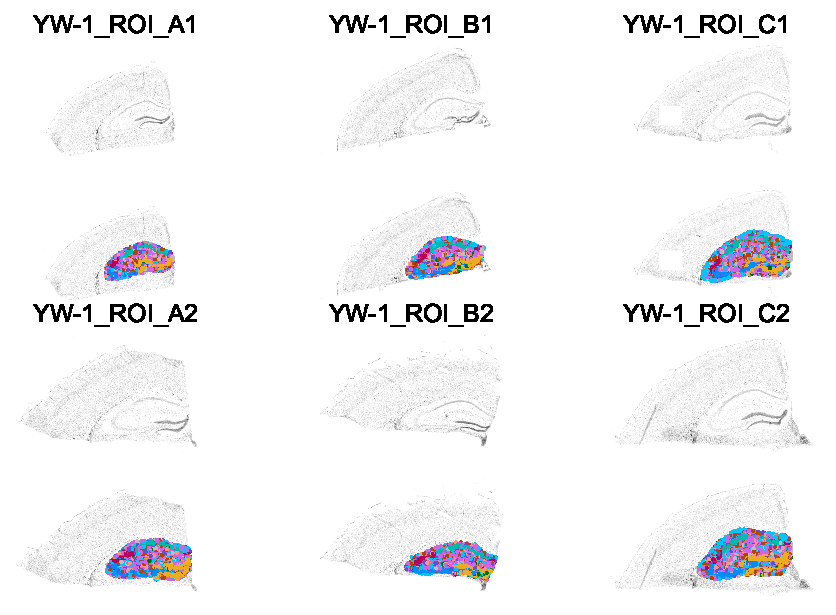
\includegraphics[width=1\textwidth]{supp_figure01_opt2_xenium_slice_clustering_all_samples_marker_size_2_resized.pdf}
\caption{Spectral clustering of all samples along with visualization of original tissue images.}

Each sample was clustered using the spectral clustering algorithm and manually labeled for the respective region or cell type. Each of the samples showed consistent clustering into the given cluster identities. 
\label{fig:clusterAllSamples}
\end{figure}

\subsection{Cell type identification}

In order to identify whether clusters were associated with a particular cell type, an analysis was performed to identify the predominant cell type in each of the remaining clusters that were not assigned to a hippocampal region. The cell types used in this analysis were: astrocytes, endothelial cells, microglia, oligodendrocytes, and neurons using gene lists from McKenzie et al. \cite{cellTypeGenetics}, as well as genes known to be identifiers for certain interneurons. The lists for each cell type in the original paper contain 1,000 genes per cell type. The genes contained in the Xenium dataset were then compared to these gene lists to identify potential marker genes within the data. All genes used are listed in \textbf{Supp. Table X} along with the corresponding cell type. Between 16 and 25 genes were used to identify each of the cell types astrocytes (20 genes), endothelial (25), microglia (16), and oligodendrocytes (16). For the interneuron cluster, five lists were curated with 4 to 8 genes each for five different types of interneurons. These included markers for Pvalb (6 genes), Sst (5), Vip (8), Sncg (4), and Lamp5 (7) interneurons. In order to identify cell types, a z-scored gene matrix was first calculated for each hippocampal sample, normalizing each gene to a mean of zero. For each cell, the mean was calculated of all genes for a particular cell type and plotted as seen in Fig. \ref{fig:cellTypeID}

With the mean z-score calculated for each set of cell-type genes, the values were plotted to the locations of the cells in each of the remaining clusters. For the sake of brevity, all clusters identified as being one of the 5 interneurons were assigned to the larger 'neuron' cluster, but these groups could be used later for more in depth analysis of the data as a whole. Each of the clusters was examined and the cell-type with the largest mean z-score across all cells was selected as the identifier. In the case that there was no clear cell-type association across all cells in a cluster, those cells were left unlabeled and not included in the statistical analysis of the clusters between NSD and SD.

\begin{figure}
\centering
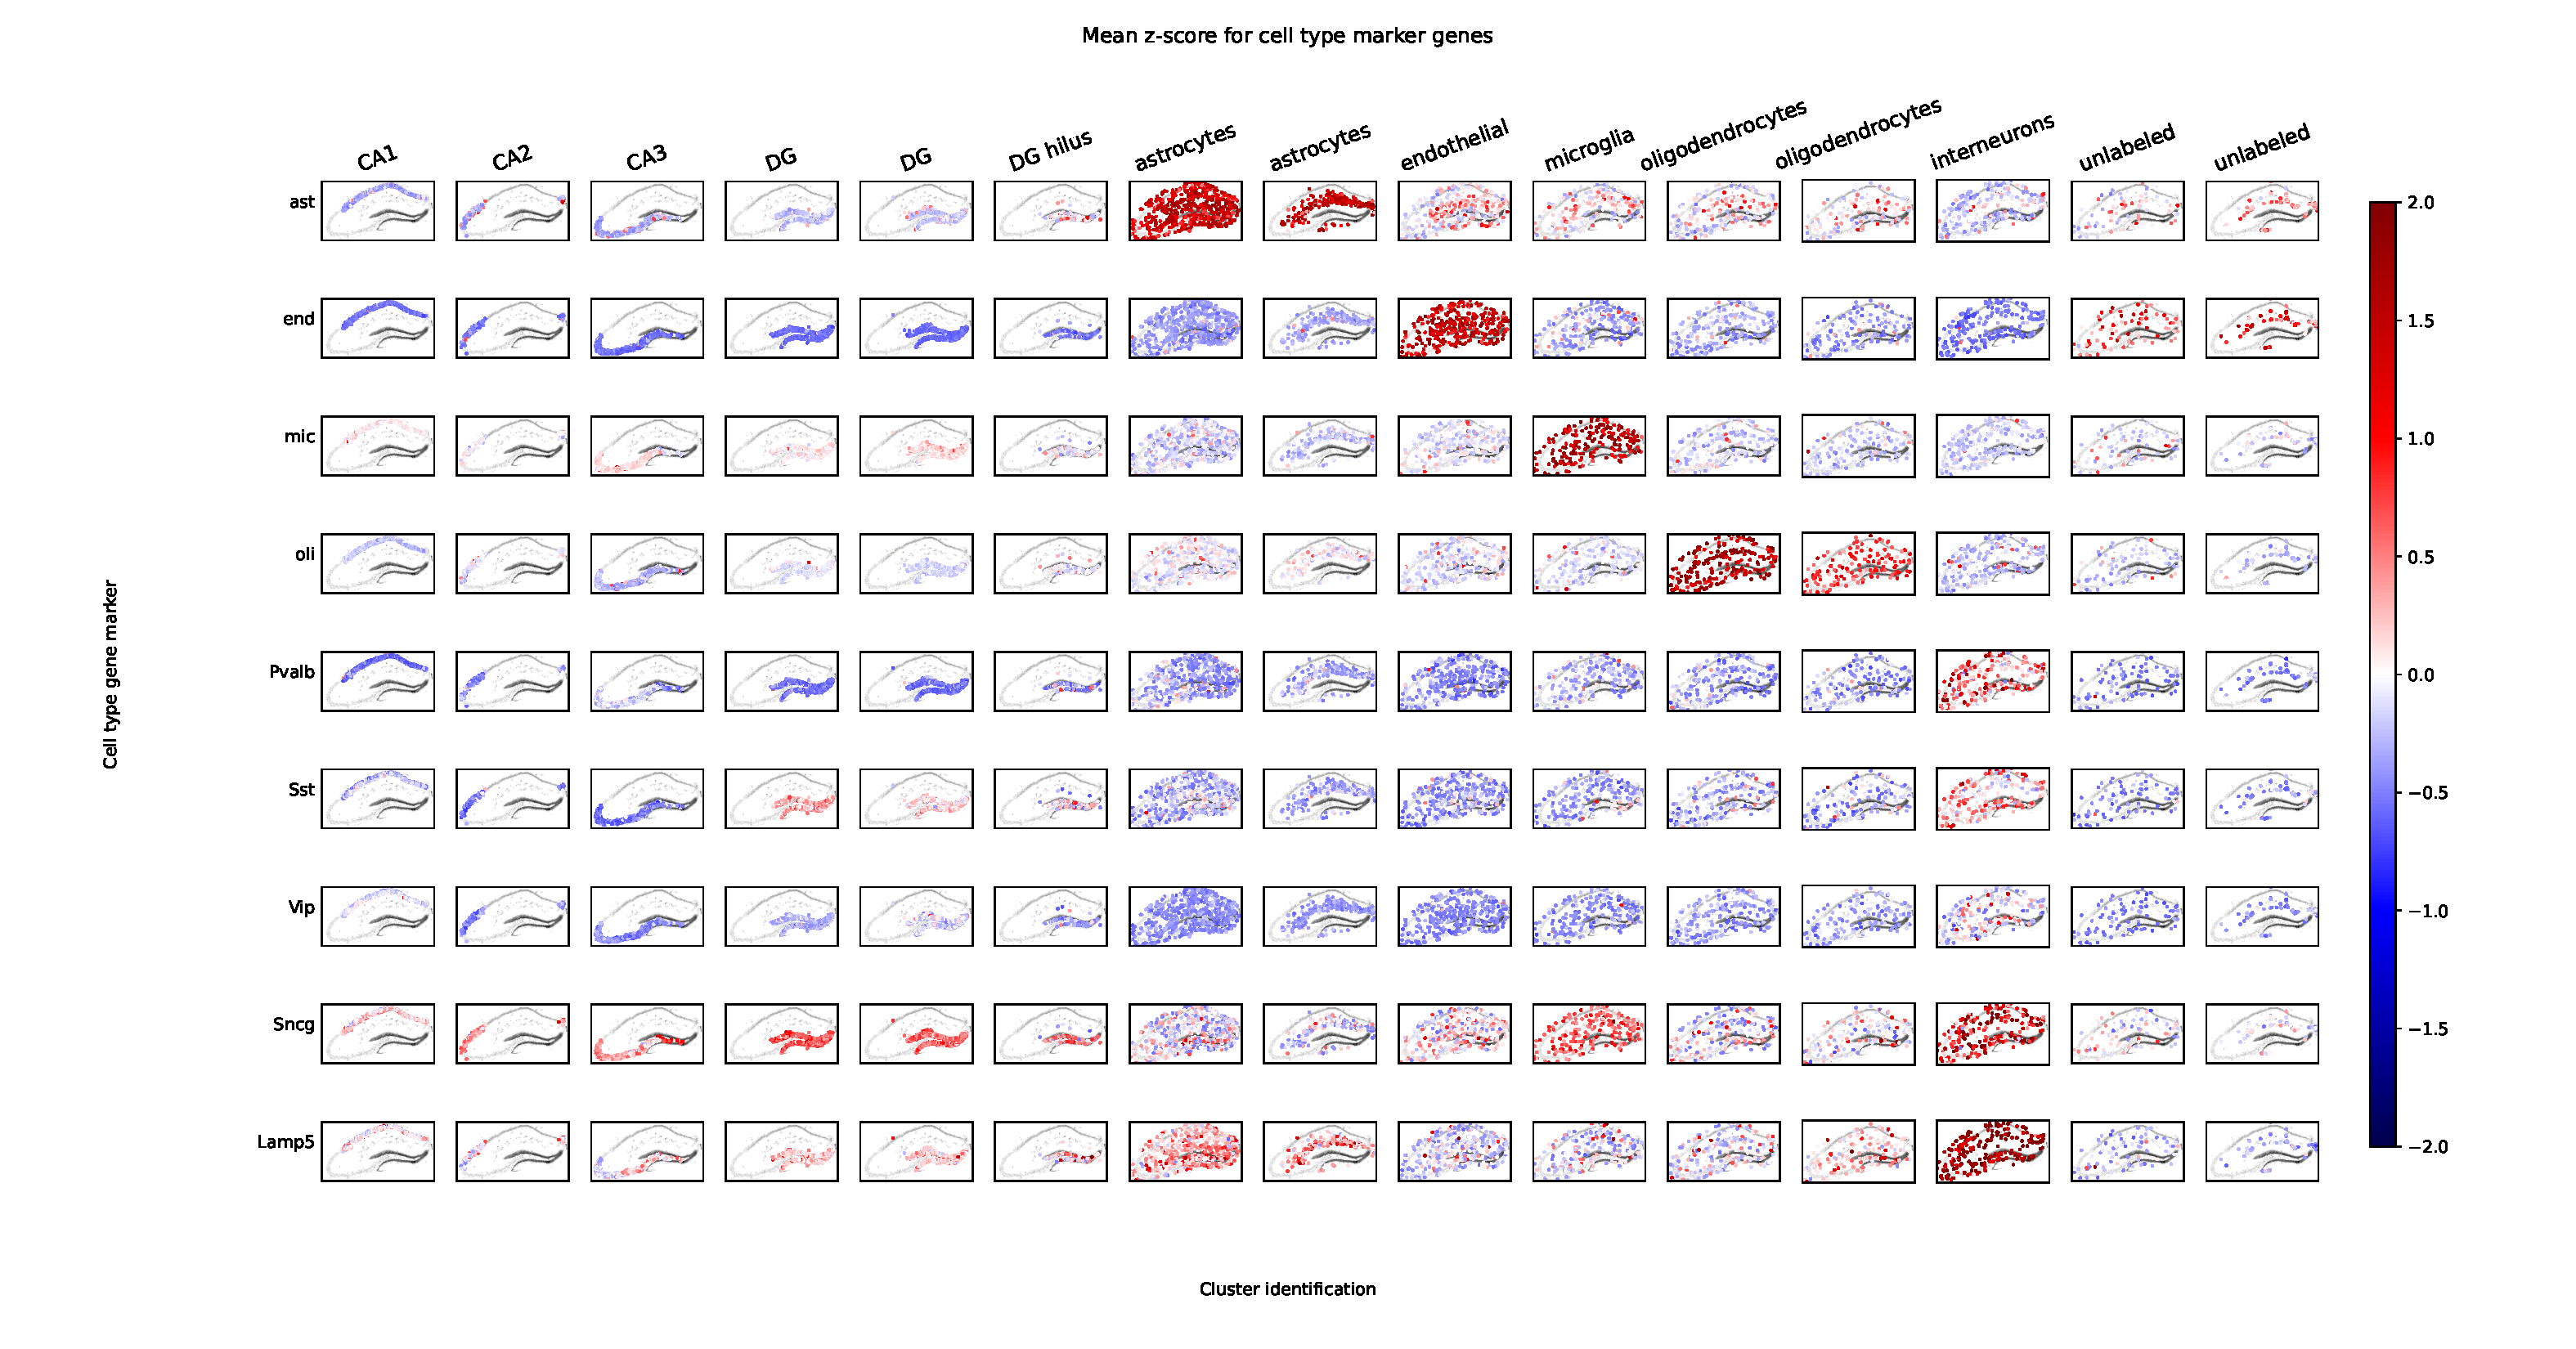
\includegraphics[width=1\textwidth]{xenium_mean_z-score_for_cell_type_marker_genes_with_interneurons_YW-1_ROI_A1_hippocampus_cluster_labels.pdf}
\caption{Mean z-score per cell for cell-type gene markers}
Shows the mean z-score for each of the sets of cell-type specific marker genes within the cells of the clusters that were not assigned to specific regional clusters, where red color indicates a positive mean z-score and blue indicates a negative mean z-score. The darker the color, the greater the z-score value in each direction. The colorbar is capped to a z-score of [-2,2].
\label{fig:cellTypeID}
\end{figure}

\subsection{Differentially expressed gene analysis}

Using the above defined cluster labels, t-tests were performed on each region. This was done by combining all cells from a given cluster in a single sample into a vector with all cells from the same cluster in the remaining samples of the same condition and performing an t-test between the $log_{2}$ normalized gene counts for NSD and SD. Benjamini-Hochberg correction was used to account for false discovery rate. Fold change was calculated using the following equation:
 
\begin{equation}
logFC = log_{2}(\frac{mean\ gene\ count\ SD}{mean\ gene\ count\ NSD})
\end{equation}

In order to plot the data, the intensity of the color is a plot of the t-statistic value. This value was applied to all cells within a given cluster and plotted as either red for a positive t-statistic or blue for a negative t-statistic. 

\section{Results}

\subsection{Clustering of Xenium data}

Each of the samples was restricted to only the cells that made up the hippocampal formation. The mean number of cells per slice was 5811.75. 

The clustering of the data showed certain consistent groupings across all samples. Three major subfields of the Cornu ammonis, the CA1, CA2, and CA3 were present in the clustering of each samples, regardless of sleep deprivation status, indicating that the transcriptomic patterns within the cells of these regions are highly specific. The dentate gyrus was broken into two clusters, one that covered the majority of the cells within the region, and another cluster that lay along the inner portion of the DG, surrounding the area that would be the CA4. For this reason, these two clusters were described as DG and DG interneurons respectively, as they consistently showed unique transcriptomic patterns causing them to be separately clustered. The remaining clusters did not have a regionally defined identity, but rather were classified based on association with cell-type specific markers. Astrocytes consistently showed strong within group association, where clusters associated with astrocytes were highly overexpressed for astrocytic markers while showing decreased expression for markers of other cell types, as seen in Supp. Fig. \ref{fig:cellTypeID}. Microglia and endothelial cells additionally showed a strong unique association for all cells within a particular cluster, making them easy to identify as unique groups. Oligodendrocytes tended to form two clusters, likely indicating oligodendrocytes and oligodendrocyte precursor cells, however for the sake of this work these two clusters were combined into one "oligodendrocyte" cluster, but this would be a good source for potential further investigation of the data. Because the list of gene markers for neurons included markers for all types of neurons, including excitatory and inhibitory, as well as various interneurons, gene lists were instead created by the authors that would identify markers for specific interneurons that are expected to be found in the hippocampus. These interneurons are listed in the methods section but also showed association across different types that allowed the combination of multiple clusters into a single "interneuron" cluster. 

The largest of the clusters based on number of cells was the dentate gyrus, containing 11,374 cells across all combined samples.The DG is known to be made up of densely packed neurons, which is confirmed by the transcriptomic based clustering \ref{table:degsPerRegion}. Within the DG interneuron cluster there were 1,506 cells. The corpus ammon regions were the next most populated regionally defined clusters, with 4,825 cells in the CA1, 1,506 in the CA2, and 3,566 in the CA3, with 88, 39, and 51 DEGs in each of these regions respectively. 

All four of the regionally defined clusters contained multiple DEGs that were specific to to the clusters, with the DG having the most unique DEGs at 34, the CA1 having 15, the CA3 having 8, and the CA2 4. For the cell type defined clusters, only two of the cell types contained unique DEGs, the astrocyte population with 29 DEGs, and the microglia with a single unique gene. 

\begin{figure}
\centering
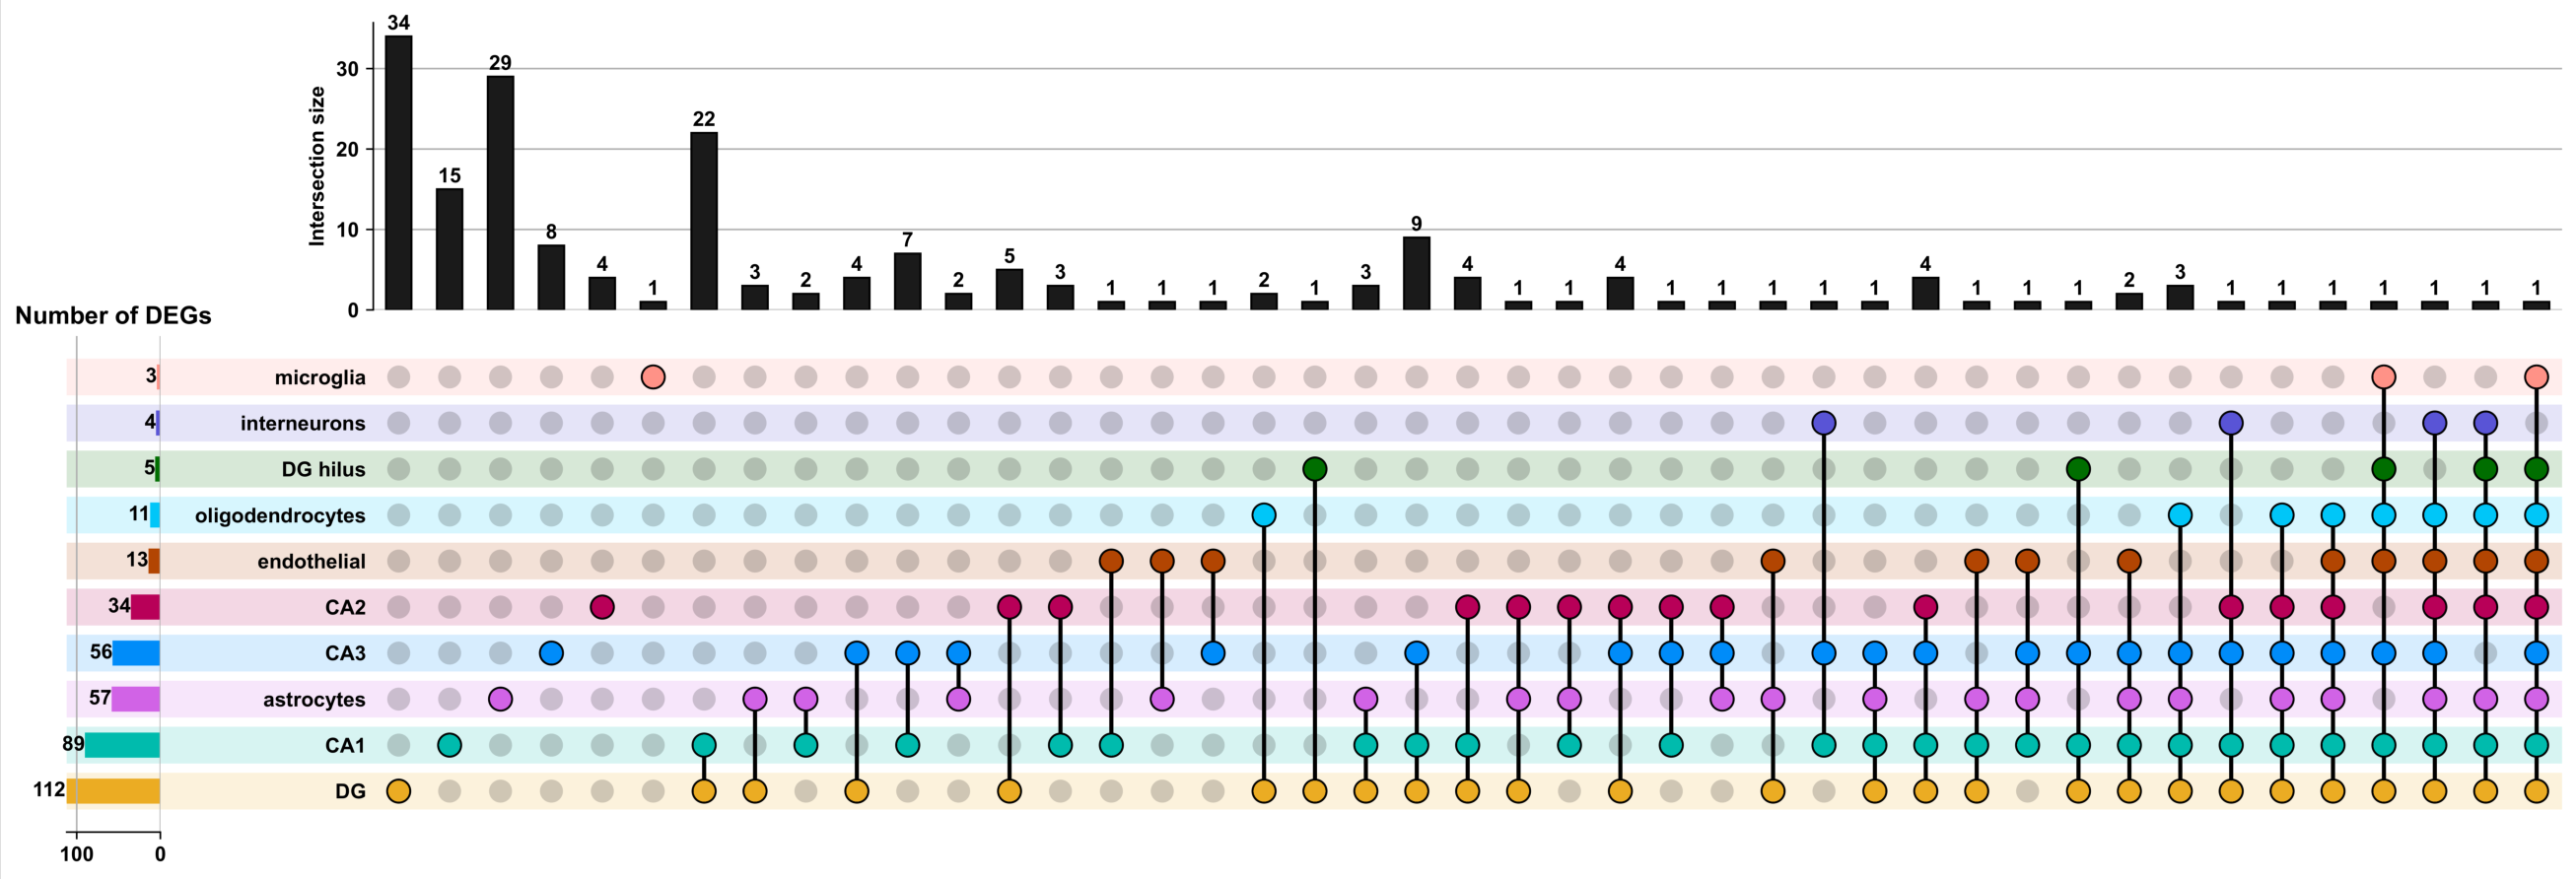
\includegraphics[width=1\textwidth]{upset_plot_of_DEGS_color_underlay_black_lines_color_spots.pdf}
\caption{UpSet plot of DEGs based on clusters and intersection}
The overlap of differentially expressed genes shared across different clusters in the analysis. The DG shows both the largest number of total DEGs as well as the largest number of unique DEGs. Astrocytes show over half of the DEGs present are unique to the astrocyte cluster, while the CA1 shows a large amount of overlap with the DEGs found in other clusters.  
\label{fig:degUpsetPlot}
\end{figure}


There were a total of six genes that were differentially expressed in at least five regions. Of those six genes, multiple prove confirmation of previous works showing differential expression. Cirbp, Rbm3, and Ttr all show broad decreased expression in the hippocampal formation. This is in line for what is known about Cirbp and Rbm3 (***Gaine, et al 2021*** for Cirbp, Visium paper for Rbm3). Ttr generally shows lower expression throughout the hippocampus, but it is more highly expressed in astrocytes, where is shows a strong decrease in expression. Previous work looking at transthyretin (Ttr) in the hippocampus showed the gene to be upregulated in stress-induced depression (Takatsuki, 2023, need to read more closely to see if actually relevant). On the other hand, Dusp5, Hspa5, and Sdf2l1 all showed increased expression following sleep deprivation.

\begin{figure}
\centering
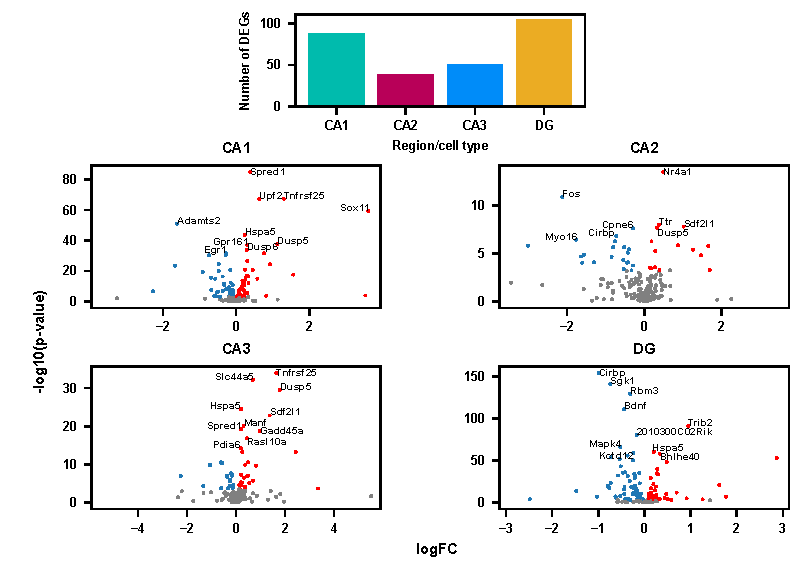
\includegraphics[width=1\textwidth]{figure02_regional_volcano_plots_volcano_marker_2_text_fixed.pdf}
\caption{Differentially expressed genes within regionally defined clusters.}
Bar graph shows the number of DEGs present in each of the regionally defined clusters. The volcano plots show the fold change and significance within each region, with the $-log_{10}(p-value)$ on the y-axis and the $logFC$ on the x-axis. The top 10 genes based on sorted p-values are listed. If less than 10 genes were significant, only the significant genes are shown. Significantly upregulated genes are displayed in red, while significantly downregulated genes are displayed in blue. 
\label{fig:volcanoPlotRegional}
\end{figure}

\begin{figure}
\centering
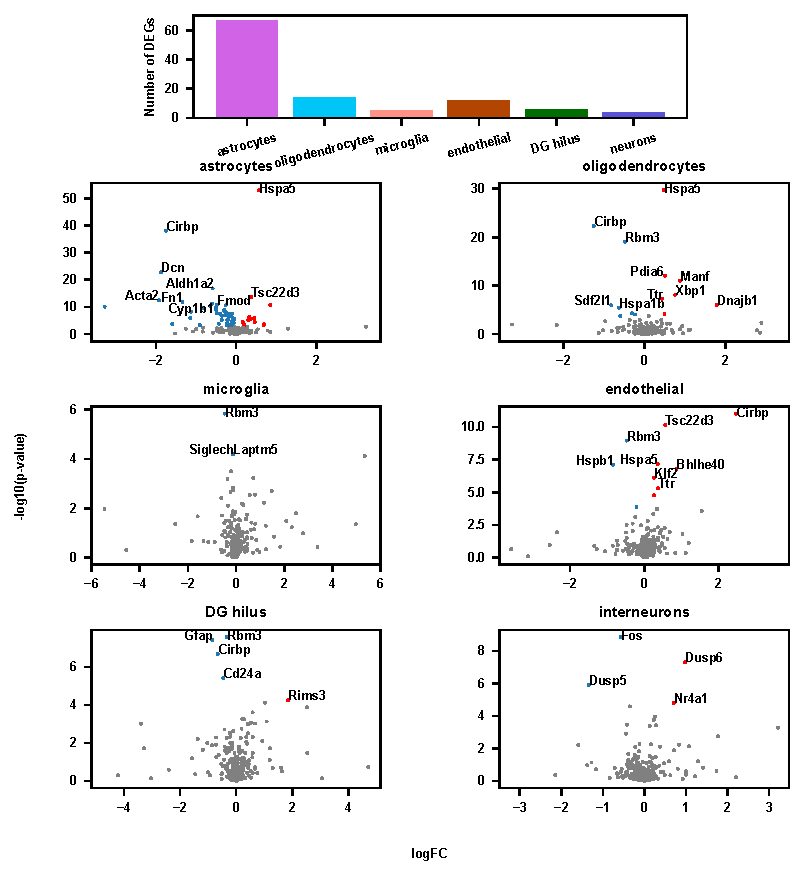
\includegraphics[width=1\textwidth]{figure03_cell_type_volcano_plots_volcano_marker_2_text_fixed.pdf}
\caption{Differentially expressed genes within cell type defined clusters.}
Bar graph shows the number of DEGs present in each of the cell type based clusters. The volcano plots show the fold change and significance within each region, with the $-log_{10}(p-value)$ on the y-axis and the $logFC$ on the x-axis. The top 10 genes based on sorted p-values are listed. If less than 10 genes were significant, only the significant genes are shown. Significantly upregulated genes are displayed in red, while significantly downregulated genes are displayed in blue. 
\label{fig:volcanoPlotCellType}
\end{figure}

\begin{table}
\begin{tabular}{|l | l | l|}
    \hline
    \textbf{Cluster name}    &	\textbf{Number of cells}	&	\textbf{Number of DEGs}    \\ \hline
	CA1	&	4,825	&	88	\\	\hline
	CA2	&	1,506	&	39	\\	\hline
	CA3	&	3,566	&	51	\\	\hline
	DG	&	11,374	&	105	\\	\hline
	DG interneurons	&	1,091	& 6	\\	\hline
	astrocytes	&	4,245	&	67	\\	\hline
	endothelial	&	1,984	&	12	\\	\hline
	microglia	&	1,068	&	5	\\	\hline
	neurons		&	1,635	&	4	\\	\hline
	oligodendrocytes	&	2,592	&	14	\\	\hline
	unlabeled	&	1,393	&	N/A	\\	\hline
\end{tabular}
\caption{Cluster labels along with the number of cells per and differentially expressed genes per cluster}
\label{table:degsPerRegion}
\end{table}

\section{Discussion}

\subsection{Differential expression between Corpus ammon regions and dentate gyrus}
One fact that becomes noticeable when examining the results of the cluster based statistics is that the different subregions of the mouse hippocampus respond differently, and in different directions, to sleep deprivation. For example, Fos, FosB, and Fosl2 which make up the Fos gene family all show increased expression in the CA1, CA2, and CA3 while showing decreased expression in the dentage gyrus. This matches with known differences between the responses of the CA1 and other portions of Ammon's horn and the DG, where the DG tends to be more resilient to external insults than the CA1 \cite{diffOfCAandDG}.


\subsection{Future directions}
It is worth noting that the dentate gyrus often generates multiple clusters in each sample, this is likely the result of the high density of cells within the region. Future directions might include specifically subdividing the dentate gyrus into multiple subregions. It is known that the DG contains various subregions, both inferior and superior DG. 

Further future directions that would be possible to investigate using spatial transcriptomic technologies would be the correlation between different subregions of the CA1 and CA3, which have been defined in relationship to spatial and non-spatial memory, but have yet to be properly defined a spatial transcriptomic analysis. 

\bibliographystyle{plain}
\bibliography{references.bib}

\end{document}

%%% sidak correction information
% clusters separately, looking for changes in gene expression across all cells between NSD and SD. Sidak correction was used to account for multiple comparisons, where an alpha of $p=0.05$ was adjusted based on the number of t-tests performed, i.e. the number of genes (Eq. 2). A gene was considered to be significantly differentially expressed if the p-value for the t-statistic was below the calculated $\alpha_s = 1.57 \times 10^{-5}$.

% \begin{equation}
% \alpha_s = 1 - (1-\alpha)^{1/N_g}
% \end{equation}


%%% cell-type gene table
% \begin{tabular}{|l | l|}
%     \hline
%     \textbf{Gene name}    &   \textbf{Cell type}    \\ \hline
% 	Aqp4		& astrocytes	\\
% 	Gli3		& astrocytes	\\
% 	Acsbg1		& astrocytes	\\
% 	Gfap		& astrocytes	\\
% 	Slc39a12	& astrocytes	\\
% 	Dio2		& astrocytes	\\
% 	Ntsr2		& astrocytes	\\
% 	Rorb		& astrocytes	\\
% 	Rmst		& astrocytes	\\
% 	Rfx4		& astrocytes	\\
% 	Hapln1		& astrocytes	\\
% 	Mapk4		& astrocytes	\\
% 	Cd44		& astrocytes	\\
% 	Pantr1		& astrocytes	\\
% 	Plch1		& astrocytes	\\
% 	Igfbp5		& astrocytes	\\
% 	Fezf2		& astrocytes	\\
% 	Fmod		& astrocytes	\\
% 	Zfpm2		& astrocytes	\\
% 	Pln			& astrocytes	\\
% 	Adgrl4		& endothelial	\\
% 	Emcn		& endothelial	\\
% 	Cd93		& endothelial	\\
% 	Nostrin		& endothelial	\\
% 	Ly6a		& endothelial	\\
% 	Fn1			& endothelial	\\
% 	Cldn5		& endothelial	\\
% 	Mecom		& endothelial	\\
% 	Kdr			& endothelial	\\
% 	Pglyrp1		& endothelial	\\
% 	Sox17		& endothelial	\\
% 	Pecam1		& endothelial	\\
% 	Acvrl1		& endothelial	\\
% 	Slc2a1		& endothelial	\\
% 	Paqr5		& endothelial	\\
% 	Slfn5		& endothelial	\\
% 	Fgd5		& endothelial	\\
% 	Hspb1		& endothelial	\\
% 	Acta2		& endothelial	\\
% 	Cobll1		& endothelial	\\
% 	Klf2		& endothelial	\\
% 	Ano1		& endothelial	\\
% 	Arhgap6		& endothelial	\\
% 	Cpne8		& endothelial	\\
% 	Gadd45a		& endothelial	\\

% \end{tabular}